%Introduction
%  Adsorbate-Metal systems 
%      catalysts
%      devices
%      oxide formation
%    This dissertation
%      structure
%      dynamics
%      reconstruction
%      accurate treatment of electronic interactions and charge transfer effects
%    Organized
%      1: Intro
%      2: Methodology Development
%      3: Pt-CO 557
%      4: Pt/Pd-CO 557
%      5: 112/557/321/765
%      6: MM-FlucQ
%      7: Summary
%
%  Metal Systems:
%      Structure
%        bimetallic (alloys, layers, near surface alloys, etc.)
%      Dynamics
%    Adsorbate Interactions:
%      binding sites
%      patterning
%    Dynamics
%      diffusion
%      step-wandering
%    Reconstruction
%      refaceting
%      doubling
%      island formation

\chapter{INTRODUCTION}
%CHAP1
%Metal surfaces
%  motivation (catalysis, energy generation, biomedical applications)
%  electronic, optical properties (stable at extreme temperatures, pressures for the most part)
%  list off neat things metal surfaces have done (20 or so spread throughout first couple of paragraphs
% Tie into importance of adsorbate interactions
Metal surfaces and nanoparticles play a role in many areas of chemistry,
including catalysis\citep{}, energy generation\citep{}, and biomedical
applications.\citep{} The differences in their displayed facets and morphologies can play a
significant role in their activity\citep{}, selectivity\citep{}, and
stability\citep{}. Bimetallic species and alloys\citep{}, along with supported
surfaces and nanoparticles\citep{} allow for an even greater design space for
various mechanical\citep{}, optical\citep{}, and catalytic properties.\citep{}
In most practical applications the surface of the metal will be exposed to a
variety of atmospheric compositions leading to adsorbed species on the surface
and potentially oxide formation. The interactions between metals and adsorbates
adds another layer of complexity when attempting to fully describe metal
surfaces.  This dissertation is intended to provide a fundamental picture for
adsorbate induced reconstruction on metal surfaces by examining the complex
interactions present in these systems, measuring the perturbed dynamics, and
analyzing the effect of different exposed facets by using Molecular Dynamics
(MD) simulations to capture the atomic mechanisms that lead to restructuring.



%In general, the structure of metal surfaces can be strongly perturbed by the
%presence of adsorbates. The extent of adsorbate coverage and the strength of
%adsorbate self-interactions can both drastically affect the predicted
%low-energy surface. If the preferred low-energy is modified and the kinetic
%barrier is not too large, surface reconstructions can result.  Since the
%efficacy of metal surfaces strongly depends on the exposed structure, having a
%detailed understanding of the mechanism of surface dynamics and restructuring
%as caused by adsorbates is of the utmost relevance. 



This dissertation is organized so that a brief overview of metallic systems,
adsorbate interactions, and adsorbate-induced reconstructions are presented in
Chapter 1. The second chapter focuses on accurately modeling the metal-metal,
metal-adsorbate, and adsorbate-adsorbate interactions, along with introducing
the multiple-minima fluctuating charge (MM-flucQ) method as it relates to the
electrostatic interactions present in the system. Chapter 3 presents work
on the surface reconstructions of Pt (557) and Au (557) surfaces when exposed
to Carbon Monoxide. In Chapter 4 the effect of CO adsorption on a Pt/Pd (557)
subsurface alloy is explored. The fifth chapter more fully examines the effects
of step type and plateau length as they affect the CO-induced restructuring of
Platinum. Moving away from Pt-CO systems, Chapter 6 presents our development of
the MM-flucQ potential and its applications to charge transfer and oxide
formation on Pt surfaces. Finally, Chapter 7 contains a summary of this
work as well as proposals for future directions.

\section{Metals}
The electronic nature of metals, as compared to other molecular species makes
them particularly interesting for a variety of chemical or material processes
where their specific characteristics can be used effectively. The ease of
movement of the valence electrons coupled with the band structure of the
molecular orbitals gives metals many technologically useful characteristics
including high electrical and thermal conductivity, malleability, and various
optical properties that make them amenable for sensing applications and energy
harvesting. While most metals have similar mechanical properties, the metals in
columns 9, 10, and 11 (Pt, Pd, Rh, etc.) of the periodic table tend to be the
most active for catalytic applications. The two primary reasons for this
phenomena are that being near the {\it d}-block these metals typically have a
larger electron density and the energy of the valence orbitals for these metals
often matches up well with adsorbate orbitals leading to strong molecular
interactions.


\begin{figure}
  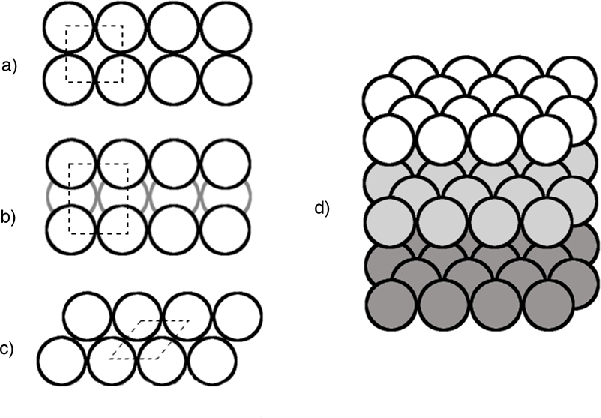
\includegraphics[width=\linewidth]{../figures/chap1/facets.pdf}
  \caption{On the left are displayed face-down views of common low-index facets
of metals (a) (100), (b) (110), and (c) (111). The dotted lines represent a
repeatable crystal unit on each facet. The light gray coloring in (b) is
illustrating the placement of that row of atoms beneath the top and bottom row.
Facet (d) displays a (112) step edge. The darker shading represents separate
terraces that are displaced by one atomic height.}
\label{fig:facets}
\end{figure}

\subsection{Structure}
The strength and type of bonding will depend on the displayed surface structure
of the metal.  Most metals adopt an FCC or HCP bulk crystal structure because
of their close-packing. A bulk sample can be cut along nearly any set of Miller
indices, however, some are more stable than others.  The three common low
energy facets are shown in Figure \ref{fig:facets}. For many metal surfaces,
Platinum and Palladium specifically, the surface energy of the (111) facet is
the most stable and barring kinetic barriers a higher-index surface will
minimize to this structure. The displayed low-energy structures are very
important when considering how the metal will interact with adsorbates because
the strength of the adsorption is typically tied to the displayed surface.

\subsubsection{Bimetallic Systems}
Since the properties and structure of metal systems are directly tied to their
electronic nature, anything that perturbs the density of states will likely
lead to deviations from bulk behavior. The presence of adsorbates or an
electron-donating or withdrawing support, i.e. \ce{Al2O3} will perturb the
system but one of the most powerful ways to design catalysts is through
combinding two or more metals together. Significant research has been directed
at examining various bimetallic systems, including heterogenous and homogeous
alloys, core-shell nanoparticles, and near surface alloys. Figure
\ref{fig:bimetallics} shows a number of examples. Since the proportion of each
metal along with its arrangment can in theory be tailored, bimetallic systems
allow for a high degree of tuning of various properties.

\begin{figure}
  \includegraphics[width=\linewidth]{../figures/chap1/bimetallics.pdf}
  \caption{Bimetallics}
\label{fig:bimetallics}
\end{figure}

\subsection{Dynamics}
Low-index facets of metals at room temperature will not undergo much movement
because they are already low on the potential energy surface. However, these
systems are also rarely used in real-world applications. High-index surfaces
and roughened nanoparticles have a larger number of low-coordinated surface
atoms that also tend to be more active for catalytic processes. The local
environment that enables them to bond strongly with adsorbates also can lead to
easier adatom formation and surface mobility. Repeated patterning, as seen in
step surfaces where a low-index plateau extends for some length and then
another layer of the metal is laid on top, like a staircase, can prove
especially useful because of the relatively easy characterization of the
surface.

\subsubsection{Diffusion \& Step-Wandering}
The two main types of movement that will occur on metals both involve adatoms.
Independent adatom movement is the type most likely to be seen as one particle
is ejected from a stable edge or terrace and then explores the plateau around
it. Since the strength of metallic bonding is tied to the number of nearest
neighbors, once an adatom is created and is seated on the surface, there is
often only a minimal energy barrier for it to continue exploring the surface. 

The second main type of movement involves cooperative adatom diffusion and is
better described as entire step-edges ``wandering'' on the surface. This
wandering is ultimately a collection of ejection and readsorbtion events of
surface metal atoms but it is more helpful to look at the collective motion
than all of the individual motions.

\section{Adsorbate Interactions on Metal Surfaces}
The majority of applications involving metals ultimately involve the metal
surface providing a favorable environment for some other reaction to occur,
whether that be oxidation of CO, production of \ce{H2} through a
water-gas-shift reaction, or some other mechanism that involves molecules
adsorbing to a surface. Having an accurate understanding of how adsorbates
interact with metal surfaces is thus of the utmost importance. 

\subsection{Binding Sites}
Generally, a surface with a lower index has less less electron density to
contribute to a potential adsorbate, weakening the strength of the binding.
However, the orbitals of the adsorbate also play a role in binding preference.
The three most common binding sites are highlighted in Figure
\ref{fig:binding}.
\begin{figure}
  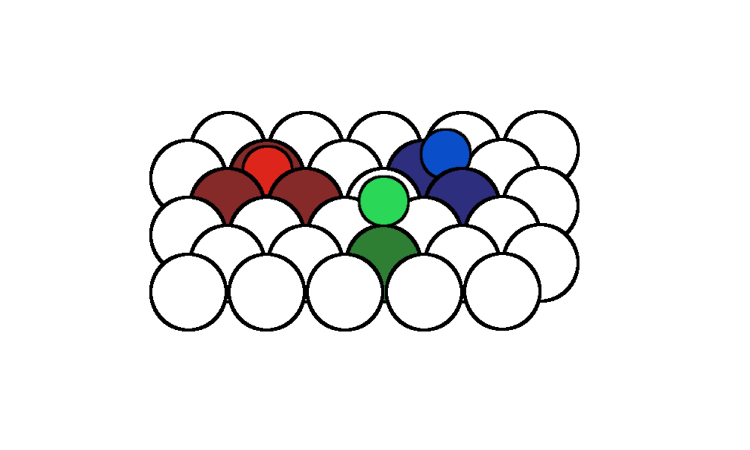
\includegraphics[width=\linewidth]{../figures/chap1/binding.pdf}
  \caption{Binding Sites}
\label{fig:binding}
\end{figure}


\subsection{Coverage Dependence}
While there might be one preferred binding site for a single adsorbate on a
metal surface, the presence of strong adsorbate-adsorbate interactions can lead
to deviations from expected behavior. While adsorbate-adsorbate interaction are
often repulsive or induce strain in the metal surface making the binding
weaker\citep{} it has been shown that cooperative effects can also arise when
adsorbates are absorbed in different electronic enivornments. It has been
predicted that while \ce{CO} prefers the atop site on \ce{Pt} at low coverages,
as the coverage approaches 0.5 monolayers the binding preference changes to a
mixed atop/bridge (CHECK) configuration because of favorable dipole-dipole
interactions that result due to non-equivalent charge transfer from the Pt back
into the CO orbitals. Since the presence and configuration of adsorbates 


\subsubsection{Patterning}
%Image of particles adsorbed on the surface
%covalent vs charge-interaction vs attractive by not strongly bound
%binding affected by surface facet (electronic, d-band) and generalized coordinate number
% sabatier/volcano plots
%experimental abilities
%dft capabilities
%where molecular dynamics fits

\section{Adsorbate Induced Reconstructions}
% Studies done on clean metal surfaces tend to suffer from pressure and temperature gaps
% high pressure xps, stm, spin echo helium bombardment provide some ways to mimic the environment of industrial catalysts
% Difficult to determine mechanisms because of time and spacial resolution
% DFT good at calculating relative energies for small systems, but the size of these reconstructions makes calculations expensive
% mol dyn. allows us to explore the interactions that lead to adsorbate-induced reconstructions

While metal surfaces often remain stable even when the environment is
perturbed, some situations can arise where the presence of adsorbates
sufficiently modify the potential energy surface so that a new facet is
energetically preferred. This situation might even be commonplace, but altering
the potential energy surface only solves part of the problem. The system must
also be able to overcome any kinetic barriers that would prevent the
restructuring from taking place. For systems that are started in a high-index
configuration, e.g. nanocubes and nanosphers, that are only is these
configuratios because of kinetic barriers, the introduction of adsorbates will
likely lead to a restructuring to a lower-energy structure. 

The time and length scales of these reconstruction processes vary
widely\citep{} and while current experimental techniques are able to observe
and identify the reconstructions, they are often unable to identify the
mechanisms of restructuring, which are important for designing catalysts.

\subsection{Refaceting}
%Williams papers on this, angle > ??? 
Surfaces will refacet if they were originally cut at too high of an angle. This
has been explored previously for a number of systems\citep{} and the refaceting
will continue until RECPLACE WITH EQUATION ABOUT STABILITY. This restructuring
typically only occurs in the forward direction while the presence of adsorbates
can induce this reconstruction, a temperature increase will also likely allow
this to occur since it is most likely that there is just a kinetic barrier that
must be overcome. 

\subsubsection{Doubling}
Work by Tao {\it et al.} on a \ce{Pt} (557) surface exposed to \ce{CO} observed
a reversible reconstruction event that was directly dependent on the presence
of \ce{CO} in the system. When \ce{CO} was introduced the step-edges doubled,
but upon removal of the \ce{CO} the original (557) motif was recovered. This
reversible reconstruction strongly implies that the presence of \ce{CO}
temporarilly modifies the potential energy surface to prefer a new ground state
structure; however, the exact mechanism of this reconstruction was not deduced
at the time. This dissertation originally started as an attempt to model this
system and attemptto provide insights into the mechanism of reconstruction. 

\subsection{Island Formation}
Since catalytic reactions typically only occur at the surface, significant
research has been devoted to increasing the surface area to bulk ratio of metal
catalysts, either through catalyst supports, high-index nanostructures, or
bimetallic near surface alloys. While these systems are typically stable at low
temperatures and pressures, significant perturbations can lead to what is
effectively sintering or island-formation of one of the metals on the surface.
The interplay of surface energies and adsorbate interactions on two or more
metal surfaces can lead to surprising results.
